\section{Introduction}
Statistical models, such as Support Vector Machines and Linear Regression, facilitate a number of important \emph{predictive} applications such as fraud detection, recommendation systems, and automatic content classification.
Increasingly, training models at scale is seen as a key data management challenge with significant interest in both industry and academia~\cite{bdas, alexandrov2014stratosphere, crotty2014tupleware, tensor}.    
Despite a number of important breakthroughs in reducing training time, constructing the statistical models on large datasets remains a tedious task due to challenges data preparation. 
Like traditional SQL analytics, statistical models are also susceptible to dirty data, including missing, incorrect, or inconsistent attributes.
Analysts widely report that this is a significant challenge~\cite{kandel2012,nytimes}, and consequently, it is important to understand the relationship between data cleaning and model training workflows.

\begin{figure}[t]
\centering
 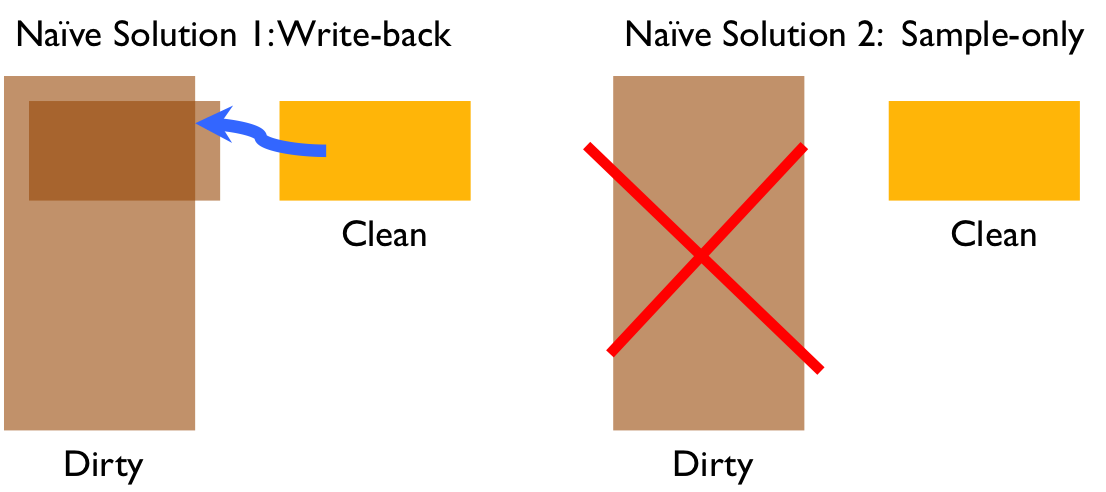
\includegraphics[width=\columnwidth]{figs/update-arch.png}
 \caption{(a) Systematic corruption in one variable can lead to a shifted model. 
 (b) Mixed dirty and clean data results in a less accurate model than no cleaning.
(c) Small samples of only clean data can result in similarly inaccurate models. \label{update-arch1}}
\end{figure}

While data cleaning has been extensively studied, the high dimensionality of typical statistical modeling problems can lead to very counter-intuitive effects.
For example, it well known that many analysts apply data cleaning iteratively--alternating between cleaning and analysis until a desired accuracy is reached.
While this procedure is intuitive for \sumfunc, \countfunc, \avgfunc aggregate queries, this process can lead to arbitrarily incorrect results for even simple statistical models in two dimensions.
Figure \ref{update-arch1}a illustrates training a linear regression on systematically biased (shifted) data.
If the analyst only partially cleans the dataset in the first iteration and re-trains the model, the intermediate result can be very incorrect (Figure \ref{update-arch1}b).
Thus, the analyst cannot use this intermediate result to make a judgement about data quality or the effects of data cleaning. 
Similarly, high dimensional models face more dramatic sampling effects than the traditional aggregates (Figure \ref{update-arch1}c).

Data cleaning is a broad problem that encompasses extraction, de-duplication, schema matching, and many other techniques.
In this paper, we focus on two forms of data cleaning that are prevalent in statistical modeling, removing outliers and attribute transformation.
For example, battery-powered sensors can transmit unreliable measurements when battery levels are low \cite{DBLP:conf/pervasive/JefferyAFHW06}. 
Similarly, data entered by humans can be susceptible to a variety of inconsistencies (e.g., typos), and unintentional cognitive biases~\cite{DBLP:conf/recsys/KrishnanPFG14}.
Since these two types of errors do not affect the schema or leave any obvious signs of corruption (e.g., NULL values), model training may seemingly succeed--albeit with an inaccurate result.

We propose \sys which is a model training framework that allows for iterative data cleaning while preserving provable convergence properties.
The analyst initializes an \sys with an ML model, a featurization function, and a pointer to the base relational data, and the \sys initially returns the model trained on the dataset.
\sys recommends a set of sample data that are possibly dirty based on measuring their impact and prediction accuracy with the current best model.
The analyst can apply value transformations and filtering operations to the sample data, and then prompt the system to iterate. 
\sys will incrementally and safely update the model (as opposed to complete retraining), and present a new sample to clean.
We propose several novel optimizations that leverage information from the model to guide data cleaning towards the records most likely to be dirty and most likely to affect the results.

From a statistical perspective, our key insight is to model the cleaning-training iteration as a form of Stochastic Gradient Descent, an iterative optimization method.
We treat the dirty model as an initialization, and incrementally take gradient steps towards the global solution (i.e., the clean model).
Our arguement ensures global convergence with a provable rate for an important class of models called \emph{convex}-loss models which include SVMs, Linear Regression, and Logistic Regression.
Convexity is a property that ensures that the iterative optimization converges to a true global optimum, and we can apply convergence arguments from convex optimization theory to show that \sys converges.

This paper describes the entire \sys architecture. However, the correctness of many of the components require detailed statistical proofs, which we have included in our extended technical report\footnote{\url{http://arxiv.org/pdf/1601.03797.pdf}}. To summarize our contributions:
\begin{itemize}[noitemsep]
\item \textbf{Correctness} (Section \ref{model-update}). We show how to update a dirty model given newly cleaned data. This update converges monotonically in expectation. For a batch size $b$ and iterations $T$, it converges with rate $O(\frac{1}{\sqrt{bT}})$. 
\item \textbf{Efficiency} (Section \ref{dist-samp}). We derive a theoretical optimal sampling distribution that minimizes the update error and an approximation to estimate the theoretical optimum.
\item \textbf{Detection and Estimation} (Section \ref{opti}). We show how \sys can be integrated with data detection to guide data cleaning towards records expected to be dirty.
\item The experiments evaluate these components on four datasets with real and synthetic corruption (Section \ref{eval}). Results suggests that for a fixed cleaning budget, \sys returns more accurate models than uniform sampling and Active Learning when systematic corruption is sparse.

%For a 5\%  systematic corruption, \sys cleans 55\% fewer records to achieve the same accuracy as an Active Learning algorithm.
\end{itemize}






